\documentclass[]{schulein}
%
\usepackage{schulinf}
\usepackage{floatflt}
\kopfDatum{\today} 
\fach{in-Z2}
\dokName{Asymetrische Verschlüsselung}
\keineSeitenzahlen
\documentclass{scrartcl}
\usepackage[utf8]{inputenc}
\usepackage[german]{babel}
\usepackage{lmodern}
\usepackage{graphicx}
\usepackage{setspace}
\usepackage{environ}
\usepackage{lipsum}
\usepackage{color}
\usepackage{setspace}
\usepackage{enumitem}
\usepackage{booktabs}
\usepackage{tabularx}
\newcolumntype{s}{>{\footnotesize}X}
\usepackage{longtable}
\usepackage{ltxtable}
\usepackage{pdflscape}
\usepackage{caption}
\captionsetup[longtable]{font={scriptsize},position=top,skip=0.5em}
\usepackage{url} 
\usepackage{float}
\setlist{leftmargin=*, label=-, nosep}
%
\usepackage[a4paper]{geometry} 
\geometry{top=25mm,left=25mm ,right=25mm, bottom=3cm} 
%\usepackage[babel,german=quotes]{csquotes}
%
% Pfad der Abbildungen
\graphicspath{ {../figures/} }
%
\setlength{\footheight}{50mm}
%\ifoot{\footnotesize  Quelle: Biologie heute 7/8, Schroedel 2006\\ Letzte Änderung: \today}
%\ofoot{Seite Nr. \luecke{1cm}}
%\ohead{Datum: \today}
%
% ----------
% ÜBERSHRIFT
% ----------
\newcommand{\Ueberschrift}[2]{
	\vskip 1.em
	\setlength{\tabcolsep}{0mm} % kein Innenrand bei Spaleten
	\begin{tabularx}{\linewidth}{lXr}
	{\Large\textbf{\textsf{#1}}} & &
	\includegraphics[scale=0.2]{#2}\\ % Logo rechtsbündig
	\hline
	\end{tabularx}
	% Spaltenabstand zurücksetzen
	\setlength{\tabcolsep}{6pt} 
}
% ----------
% HINWEISBOX
% ----------
\NewEnviron{hinweisbox}[2]{%
\par
\vspace{1em}
\noindent
\begin{tikzpicture}[]
	\node[rectangle,minimum width=1.0\textwidth, inner sep=0pt] (m) {
		\begin{minipage}{\textwidth}
			\dimen0\linewidth
			\advance\dimen0 by -3.0em
    			\vskip .8em \hspace{1em}
    			\parbox{\the\dimen0}{
        			\BODY\vskip .5em}%			
		\end{minipage}
		};
	\draw[#2, very thick, rounded corners, color=#1] (m.south west) rectangle (m.north east);
\end{tikzpicture}
}
%
% =======================
% Abbildungstext anpassen
% =======================
\usepackage[font={small}, labelfont=bf,figurename=Abb.]{caption}
%
% ----------
% AUFGABENBOX
% ----------
\NewEnviron{aufgabenbox}[2]{%
\par
\vspace{1em}
\noindent
\begin{tikzpicture}[]
	\node[rectangle,minimum width=1.0\textwidth, inner sep=0pt] (m) {
		\begin{minipage}{\textwidth}
			\dimen0\linewidth
			\advance\dimen0 by -3.0em
    			\vskip .8em \hspace{1em}
    			\parbox{\the\dimen0}{
        			\BODY\vskip .5em}%			
		\end{minipage}
		};
	\draw[solid, thin, color=black] (m.south west) rectangle (m.north east);
\end{tikzpicture}
}
%
% =====================================
% Litteraturverzeichnis und son kram...
% =====================================
\usepackage{url}
\usepackage[hidelinks]{hyperref}
% BibLaTeX
\usepackage[
style=authoryear-icomp,    % Zitierstil authoryear-icomp authoryear,natbib=true
isbn=false,                % ISBN nicht anzeigen, gleiches geht mit nahezu allen anderen Feldern
pagetracker=true,          % ebd. bei wiederholten Angaben (false=ausgeschaltet, page=Seite, spread=Doppelseite, true=automatisch)
maxbibnames=50,            % maximale Namen, die im Literaturverzeichnis angezeigt werden (ich wollte alle)
maxcitenames=2,            % maximale Namen, die im Text angezeigt werden, ab 4 wird u.a. nach den ersten Autor angezeigt
autocite=inline,           % regelt Aussehen für \autocite (inline=\parancite)
block=space,               % kleiner horizontaler Platz zwischen den Feldern
backref=false,              % Seiten anzeigen, auf denen die Referenz vorkommt
backrefstyle=three+,       % fasst Seiten zusammen, z.B. S. 2f, 6ff, 7-10
date=short,                % Datumsformat
]{biblatex}
\setlength{\bibitemsep}{1em}     % Abstand zwischen den Literaturangaben
\setlength{\bibhang}{2em}        % Einzug nach jeweils erster Zeile
% Heading Literaturverzeichnis anpassen
%\defbibheading{lit}{\part*{Literaturverzeichnis}
%	\markboth{\MakeUppercase{\refname}}{\MakeUppercase{\refname}}
%}
\bibliography{bib.bib}
%
% ----------
% StickyNote
% ----------
%\usepackage{xparse}
\usepackage{fancypar}
\usetikzlibrary{shadows}
\definecolor{myyellow}{RGB}{242,226,149}
\makeatletter
\pgfdeclareshape{note}{
\inheritsavedanchors[from=rectangle] % this is nearly a rectangle
\inheritanchorborder[from=rectangle]
\inheritanchor[from=rectangle]{center}
\inheritanchor[from=rectangle]{north}
\inheritanchor[from=rectangle]{south}
\inheritanchor[from=rectangle]{west}
\inheritanchor[from=rectangle]{east}
% ... and possibly more
\backgroundpath{% this is new
% store lower right in xa/ya and upper right in xb/yb
\southwest \pgf@xa=\pgf@x \pgf@ya=\pgf@y
\northeast \pgf@xb=\pgf@x \pgf@yb=\pgf@y
% compute corner of ‘‘flipped page’’
\pgf@xc=\pgf@xb \advance\pgf@xc by-10pt % this should be a parameter
\pgf@yc=\pgf@yb \advance\pgf@yc by-10pt
% construct main path
\pgfpathmoveto{\pgfpoint{\pgf@xa}{\pgf@ya}}
\pgfpathlineto{\pgfpoint{\pgf@xa}{\pgf@yb}}
\pgfpathlineto{\pgfpoint{\pgf@xc}{\pgf@yb}}
\pgfpathlineto{\pgfpoint{\pgf@xb}{\pgf@yc}}
\pgfpathlineto{\pgfpoint{\pgf@xb}{\pgf@ya}}
\pgfpathclose
% add little corner
\pgfpathmoveto{\pgfpoint{\pgf@xc}{\pgf@yb}}
\pgfpathlineto{\pgfpoint{\pgf@xc}{\pgf@yc}}
\pgfpathlineto{\pgfpoint{\pgf@xb}{\pgf@yc}}
\pgfpathlineto{\pgfpoint{\pgf@xc}{\pgf@yc}}
}
}
\makeatother
%\setlist{leftmargin=*,itemsep=4pt,parsep=0pt}
%\renewcommand{\labelitemi}{-}
%
\NewDocumentCommand\StickyNote{O{6cm}mO{6cm}O{0}}{%
\begin{tikzpicture}
\node[
note,
draw,
drop shadow={
  shadow xshift=2pt,
  shadow yshift=-4pt
},
inner xsep=7pt,
fill=myyellow,
rotate=#4,
inner ysep=10pt
] {\parbox[t][#1][c]{#3}{#2}};
\end{tikzpicture}%
}

\NewDocumentCommand\StickyNotePi{O{6cm}mO{6cm}O{0}}{%
\begin{tikzpicture}
\node[
note,
draw,
fill=myyellow,
inner xsep=10pt,
rotate=#4,
inner ysep=0pt,
text depth=\the\dimexpr#1+2.5ex\relax
] {\parbox[t][#1][c]{#3}{#2}};
\end{tikzpicture}%
}
%
% -----------
% Schriftstil
% -----------
%\renewcommand\familydefault{\sfdefault}
%
\begin{document} 
%\
\section*{Ein Verschlüsselungsverfahren entwickeln}
\subsection*{Szenario}
Alice und Bob möchten eine geheime Botschaft austauschen. Sie haben jeweils ein Schloss mit passendem Schlüssel zur Verfügung. Alice hat zusätzlich noch einen Briefumschlag für das Verschicken der Nachricht.

\Ueberschrift{Arbeitsauftrag}{pa}
\par
Simulieren Sie den Nachrichtenaustausch zwischen Alice und Bob. Entwickeln Sie dazu ein geeignetes Verschlüsselungsverfahren aus- schließlich mit den Ihnen zur Verfügung gestellten Hilfsmitteln.

\textbf{Ziel:} Der Postbote darf die Nachricht nicht mitlesen. (Trotzdem muss Bob die Nachricht entschlüsseln können!)

\begin{minipage}{.5\textwidth}
\subsection*{Regeln}
\begin{smallitemize}
\item Sie müssen die verschlüsselte Nachricht dem \glqq Postboten\grqq\ übergeben. Dieser liefert die Nachricht aus.
\item Sie dürfen sich vorab persönlich treffen.
\item Sie dürfen \textbf{nicht} die Nachricht persönlich übergeben. (Persönliche treffen dienen nur dem Austausch über das anzuwendende Verfahren).
\end{smallitemize}
\end{minipage}
\begin{minipage}{.5\textwidth}
\begin{tabular}{ccc}
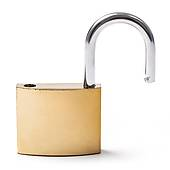
\includegraphics[width=2.1cm,clip,trim=0cm .4cm 0cm 0cm]{schloss} & 
%\hspace*{.5cm}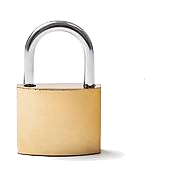
\includegraphics[width=2.5cm,clip,trim=0cm .4cm 0cm 0cm]{schloss_2}&

\includegraphics[width=2.1cm]{umschlag}&
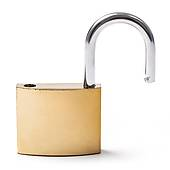
\includegraphics[width=2.1cm,clip,trim=0cm .4cm 0cm 0cm]{schloss} \\
\hspace*{-.7cm}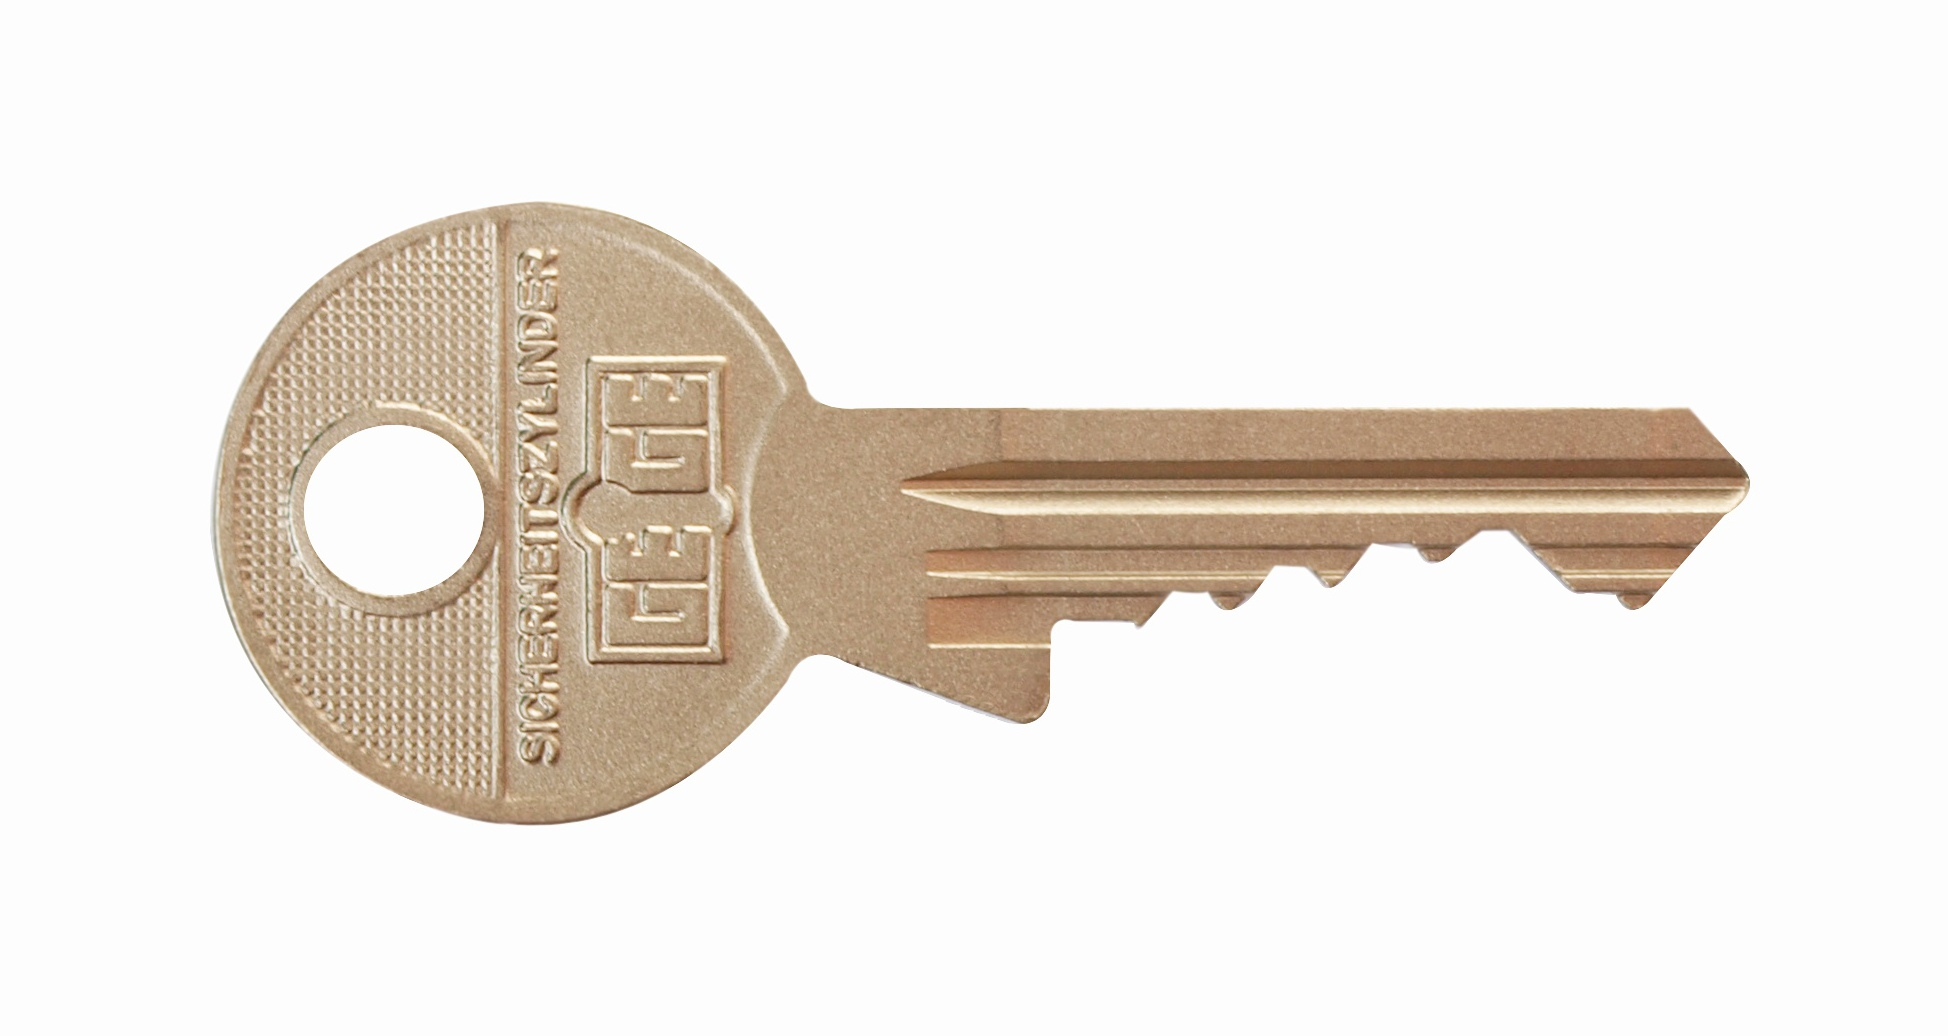
\includegraphics[angle=90,width=.8cm,clip,trim=1cm 2cm 30cm 2cm]{key}& &
\hspace*{-.7cm}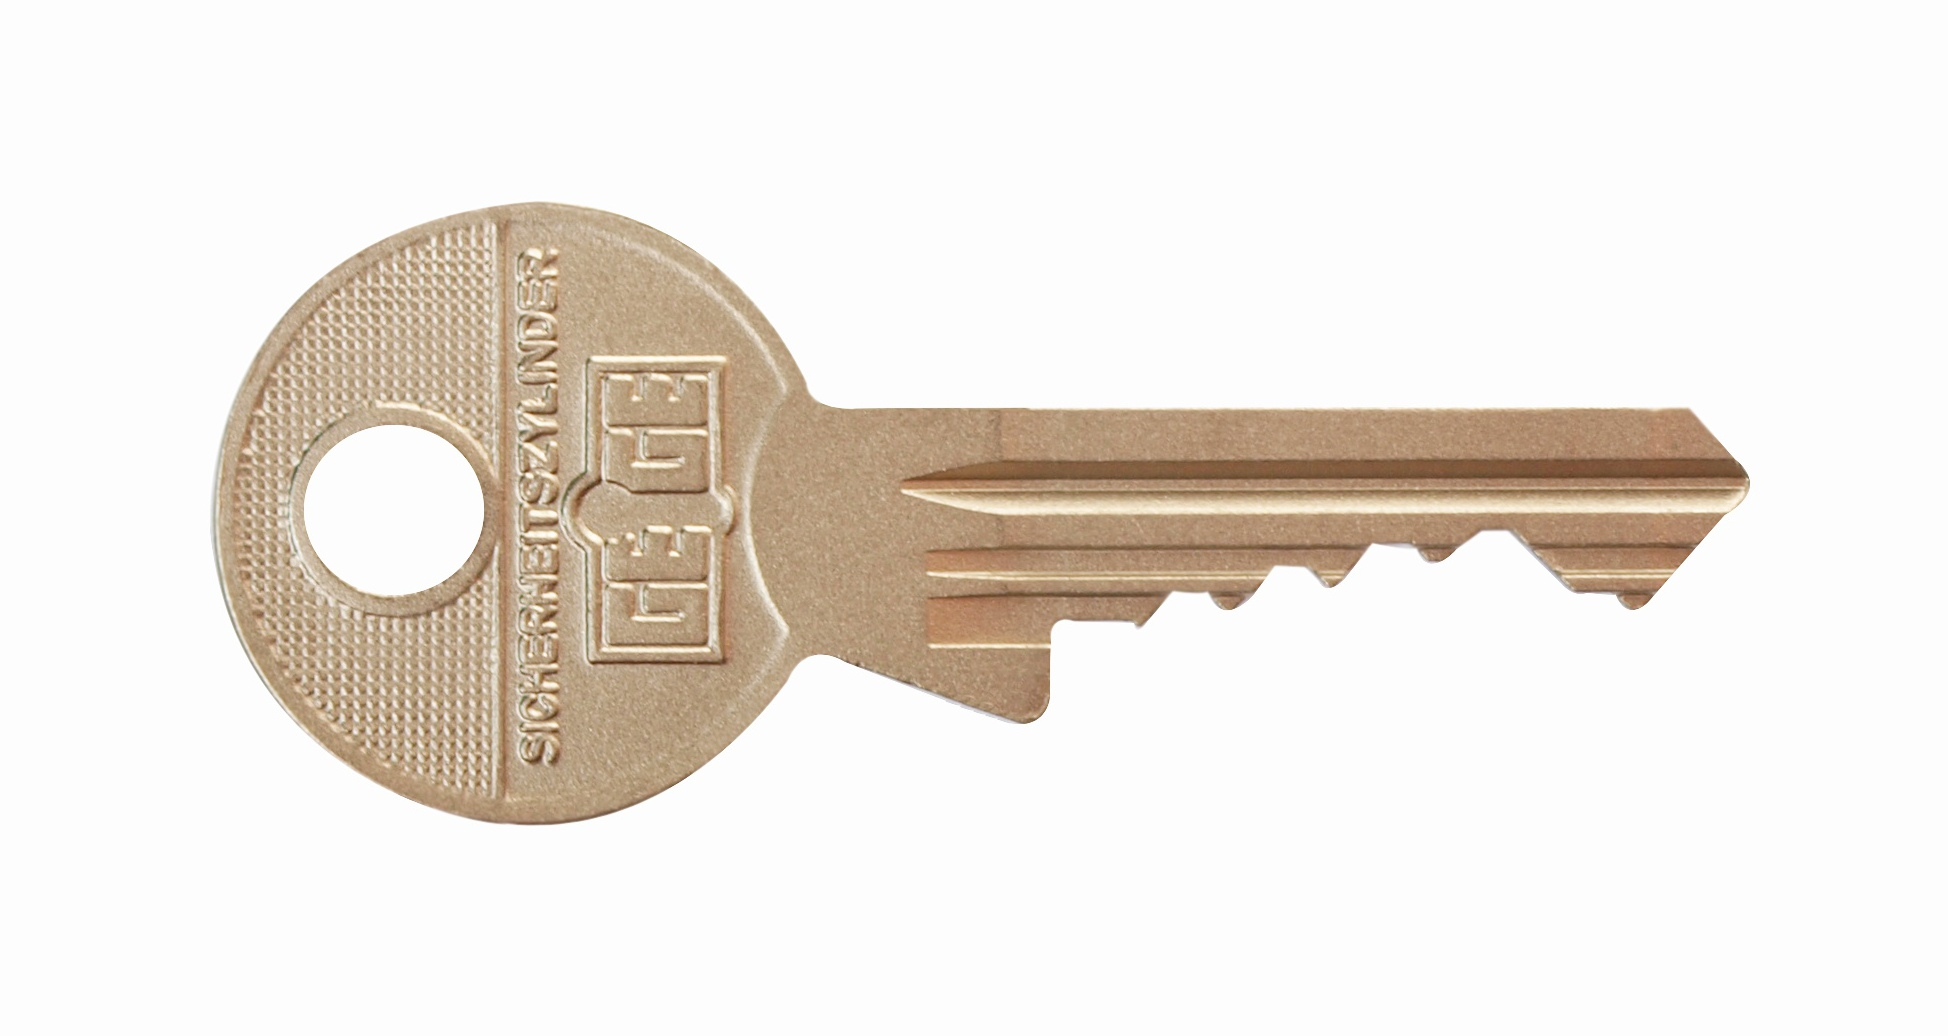
\includegraphics[angle=90,width=.8cm,clip,trim=1cm 2cm 30cm 2cm]{key}
\end{tabular}
\end{minipage}

\section*{Lösungsvorschlag (Stichpunkte)}
\end{document}